\chapter{Знакомство и первые шаги}
Эта глава посвящена первому знакомству с возможностями, которые Вам открывает Mathpar.
Язык Mathpar, который описывается ниже, может рассматриваться, как некоторое развитие языка TeX.
Язык TeX предназначен для записи математических текстов и подготовке их к публикации.
Его можно считать пассивным по сравнению с языком Mathpar, который позволяет делать вычисления,
то есть является активным языком математики. Как формулировка задачи,
так и результаты вычислений, записываются на языке Mathpar.

Сразу после вычислений Вы видите весь математический текст в виде pdf-изображения,
в том виде, как принято представлять математическую запись в научных и технических публикациях.

Этот результат может быть использован дальше несколькими способами.
 
(1) Можно кликнуть по тексту мышкой, и он вернется к исходному виду языка Mathpar.
Есть и другой способ переключения изображения текста: при помощи кнопки%begindelete
<<
\includegraphics[scale=0.6]{pictures/button_arrows.png}>>%enddelete
, расположенной между кнопками <<$\blacktriangleright$>> и <<$+$>>.

(2) Можно кликнуть по {\bf изображению математической записи} правой кнопкой мышки.
В этом случае появится выпадающее меню. Верхнее поле <<Show Math As>> позволяет
перейти к выбору  языка вывода. Предлагается выбрать TeX или MathML.
И затем открыть поле с желаемым текстом.

Например, матрица A, размера $2\times 2$, в Mathpar будет записана так:

A=[[a, b], [c, d]];

в TeX она выглядит так:

A= $\backslash$left(\comm{begin}{\{array\}}\{${cc}$\}$ a \& b$ $\backslash\backslash c \& d \backslash\backslash$ \comm{end}{\{array\}}$\backslash$right).

В MathML это еще более громоздкое выражение.
 
Полученный текст на языке TeX или MathML можно скопировать и поместить  в TeX- 
или html-файл и использовать для публикации. Кроме того, можно получить обычное 
изображение и разместить его в любом документе. Это необходимо, например, 
когда требуется сохранить график функции или решение задачи.


\section{Ввод данных,  решение задачи}

В  центральной части экрана находится поле ввода. Здесь Вы размещаете математические выражения.  
Для решения задачи надо нажать на кнопку <<${\blacktriangleright}$>>, которая 
расположена над полем ввода. Кроме того, можно использовать сочетание клавиш {\it Ctrl+Enter}. 
Например, можно набрать 2+2 и нажать <<$\blacktriangleright$>>.

В верхней части экрана находятся активные поля $\fbox{Помощь}$ и $\fbox{Руководство}$. 
Указывая мышкой на эти поля, Вы можете перейти к страницам Помощи или открыть Руководство по языку Mathpar.

%begindelete
На рисунке приведен пример простого задания.  
 
 \begin{figure}
 \label{1_1}
\begin{center}
   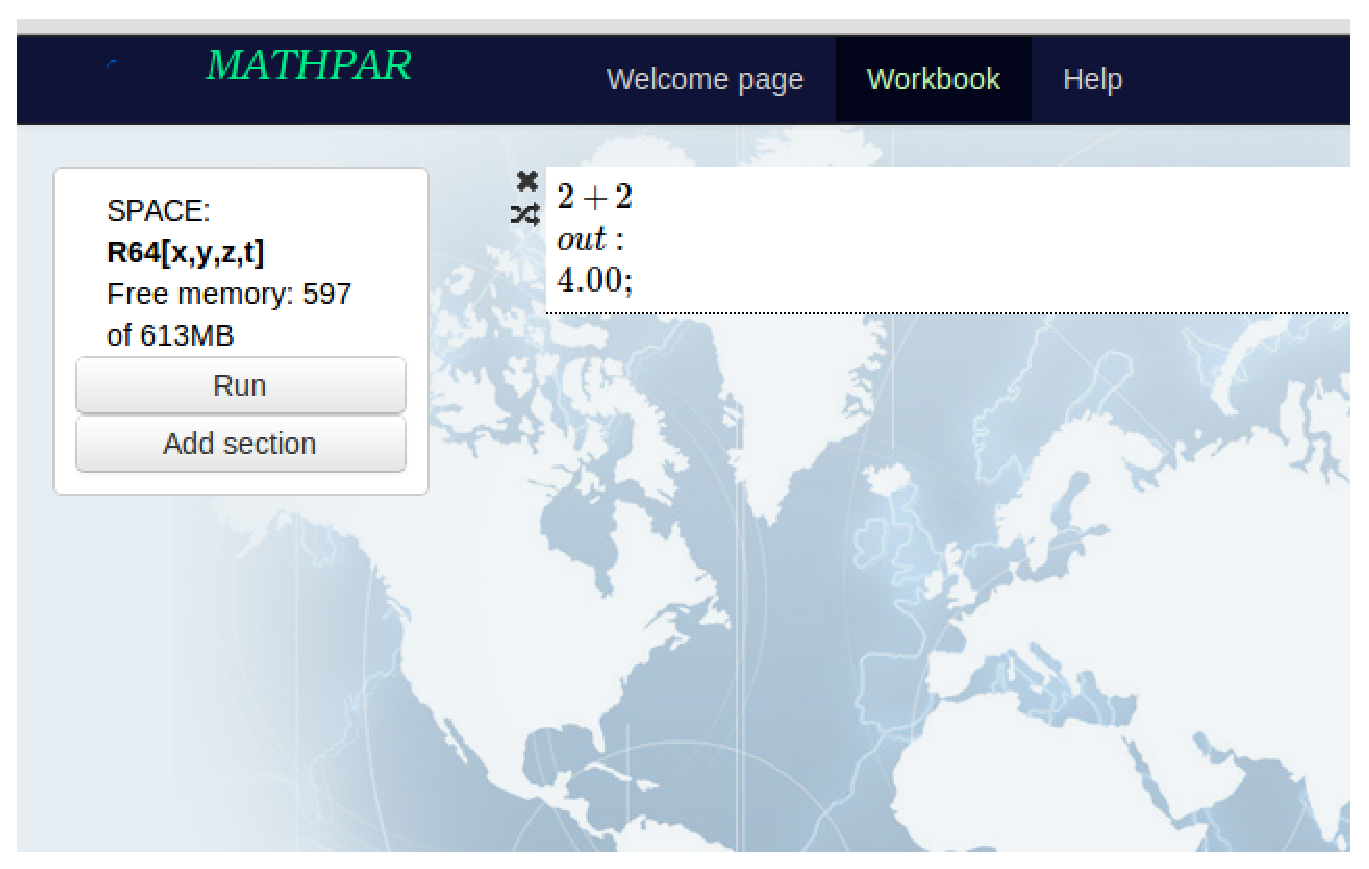
\includegraphics[scale=0.5]{pictures/1_1}
\end{center}
 \caption{Запись задания в поле ввода}
 \end{figure}
%enddelete

На страницах Помощи все поля с примерами являются активными полями, 
содержащиеся там задачи можно тут же решить и увидеть ответ.  
Для этого  нужно кликнуть по кнопке <<$\blacktriangleright$>> или же можно 
поставить курсор на поле примера и нажать {\it Ctrl+Enter}. 
Можно копировать текст из любого примера и перенести его в Ваше основное поле ввода. 
Для этого можно использовать выделение текста мышкой, копирование и вставку этого текста 
с помощью сочетания клавиш {\it Ctrl+С} и {\it Ctrl+V}, соответственно, для копирования и вставки.

Текст, который Вы можете вводить в поле ввода, состоит из комментариев и математических операторов.

При вводе комментариев, то есть любого поясняющего текста, необходимо брать его в кавычки. 
Например: ($"$ это комментарий $"$). Кавычки разрешается использовать только для комментариев. 
В тексте комментариев можно использовать, например, такие кавычки  <<  >>. 
Когда в комментариях нужно иметь математическое выражение, как часть комментария, 
то его необходимо окаймить знаками доллара ($\$$). Например, можно написать такой комментарий: \\
$"$Два обозначения $\$ \backslash exp(x)\$$  и  $\$\backslash e  \widehat{\ }{} x\$$ 
применяются для экспоненциальной функции.$"$

При вводе математических выражений их необходимо разделять точкой с запятой (;) 
или текстом комментариев, которые заключены в кавычки. Можно не ставить 
точку с запятой после последнего оператора. В математических операторах, 
когда необходимо вставить текст, нужно использовать апострофы: ('текст в математическом операторе' ).

Для вывода результатов можно использовать команду \comm{print}{()}, 
где в качестве аргументов,  разделенных запятыми,  необходимо указать имена 
тех выражений, которые требуется вывести.  Если среди команд не встретился 
оператор печати \comm{print}{()} или какой-нибудь другой оператор вывода (\comm{plot}{()}, 
\comm{prints}{()} и т. д.), то будет выводится результат, полученный в последнем 
операторе или последней новой переменной.

Команды и операторы начинаются с символа <<back slash>> ($\backslash$). 

Кнопка $\fbox{+}$ предназначена для добавления полей ввода. Для удаления поля ввода 
можно воспользоваться сочетанием клавиш {\it Ctrl+Del} или крестиком  $\fbox{х}$, 
расположенным над полем ввода справа.  

Кнопка $\fbox{C}$, расположенная над полем ввода справа, предназначена 
для отмены всех введенных раннее обозначений.     
Отмена обозначений позволяет получать формулы, в которых стоят символы, а не числа.

В левой верхней части экрана находятся поля, в которых указано текущее окружение 
и объем оперативной памяти в мегабайтах. Окружение фиксируется числовым множеством 
и именами основных переменных. Под этим полем расположены различные меню, 
которые облегчают ввод функций и операторов.


\subsection{Работа с файлами}
Функции для работы с файлами доступны из раскрывающейся панели «Файлы», расположенной в меню слева.

Существуют следующие возможности для обработки файлов:

1) Сохранение последней выполненной секции в виде файла PDF с помощью
кнопки «Сохранить PDF». Можно указать собственный размер страницы (в сантиметрах),
по умолчанию указан размер А4 (21х29.7 см).

2) Загрузка текстовых файлов на сервер Mathpar с помощью кнопки «Загрузить файл».
Под этой кнопкой расположен список загруженных файлов. Файлы должны содержать выражения 
на языке Mathpar или таблицы в специальном формате.

Таблица состоит из строки с заголовком (произвольные строки) и строк с числами.
Столбцы отделяются знаком табуляции. Функции для работы с таблицами доступны 
в разделе «Графики и таблицы» (см. также раздел 3.1 Построение графиков функций 
системы помощи).

3) Ввод выражений на языке Mathpar из загруженного файла с помощью функции \comm{fromFile}{()}.
Например, создать выражение из загруженного файла myfile.txt и присвоить 
это выражение переменной $a$ можно командой a = \comm{fromFile}{('myfile.txt')}.


\section{Математические функции}
Приняты следующие обозначения для элементарных функций и констант.

\subsection{Константы}
\hspace*{4mm}  $\backslash$i --- мнимая единица,

$\backslash$e --- основание натурального логарифма,

$\backslash$pi --- число $\pi$,  то есть отношение длины окружности к диаметру,

$\backslash$infty -- знак бесконечности.


\subsection{Функции одного аргумента}

\hspace*{4mm} $\backslash$ln --- натуральный логарифм, 

 $\backslash$lg --- десятичный логарифм, 

 $\backslash$sin --- синус, 

 $\backslash$cos --- косинус, 

 $\backslash$tg --- тангенс, 

 $\backslash$ctg --- котангенс, 

 $\backslash$arcsin --- арксинус, 

 $\backslash$arccos --- арккосинус, 

 $\backslash$arctg --- арктангенс, 

 $\backslash$arcctg --- арккотангенс, 

 $\backslash$sh --- синус гиперболический, 

 $\backslash$ch --- косинус гиперболический, 

 $\backslash$th --- тангенс гиперболический, 

 $\backslash$cth --- котангенс гиперболический, 

 $\backslash$arcsh --- арксинус гиперболический, 

 $\backslash$arcch --- арккосинус гиперболический, 

 $\backslash$arcth --- арктангенс гиперболический, 

 $\backslash$arccth --- арккотангенс гиперболический, 

 $\backslash$exp --- экспонента, 

 $\backslash$sqrt --- корень квадратный, 

 $\backslash$abs --- абсолютное значение для действительных чисел,  модуль для комплексного числа,

 $\backslash$sign --- знак числа. Возвращает 1, 0,  -1,  когда число положительное, ноль или отрицательное,  соответственно,

 $\backslash$unitStep$(x)$ --- это функция, которая при $x\geqslant 0$ принимает значение $1$, а
при $x<0$ принимает значение $0$;

 $\backslash$fact --- факториал.  Определен для целых положительных чисел. Равносильная запись~--- <<n!>>.


\subsection{Функции двух аргументов}

\hspace*{4mm}  $\widehat{\ }{}$ --- степень,

 $\backslash$log --- логарифм от функции по указанному основанию,

 $\backslash$rootOf(x, n) --- корень степени n из x,   

 $\backslash$Gamma --- функция Гамма,

 $\backslash$Gamma2 --- функция Гамма 2,

 $\backslash$binomial --- число сочетаний. 


\smallskip

\underline{Примеры. }

\vspace*{-3mm}
\begin{verbatim}
SPACE = R64[x, y];
f1 = \sin(x);
f2 = \sin(\cos(x + \tg(y)));
f3 = \sin(x^2) + y;
\print(f1, f2, f3);
\end{verbatim}

%begindelete
\vspace*{-3mm}
Результат выполнения:\\
$SPACE=R64[x,y];$\\
$f1 = sin(x); $\\
$f2 = sin(cos(x+tg(y))); $\\
$f3 = sin(x^{2})+y. $
%enddelete


\section{Действия с функциями}

Для перечисленных выше функций и их композиций можно вычислить значение функции в точке,  подставить выражения в функцию вместо аргументов,  вычислить предел функции,  ее производную.  Для этого определены следующие команды. 

 
Для вычисления значения функции в точке необходимо выполнить команду \\
\comm{value}{(f, [var1, var2,\ldots, varn])}, 
где $f$~---  функция,  а $var1, var2, \ldots, varn$~--- значения соответствующих переменных кольца. 
 Для подстановки выражений в функцию необходимо выполнить команду \\
\comm{value}{(f, [func1, func2, \ldots,  funcn])},  где $f$~--- это функция,  
$func1, func2, \ldots,  funcn$~--- функции,  которые подставляются вместо соответствующих переменных. 

 Для вычисления предела функции в точке необходимо выполнить команду \\
\comm{lim}{(f, var)},  
где $f$~--- это  функция,  а $var$~--- точка,  в которой требуется найти предел. 

 Для вычисления производной функции $f$ по переменной $y$ из кольца $\mathbb{Z}[x,\ y,\ z]$
 необходимо выполнить команду  \comm{D}{(f, y)}.  Для нахождения смешанной производной первого порядка от функции $f$ существует команда 
\comm{D}{(f, [x, y])},  для нахождения производной высших порядков нужно использовать команду $\backslash {\mathbf {D}} (f, [x \widehat{\ }{} k, z \widehat{\ }{} m, y \widehat{\ }{} n])$,  где $k,  m,  n$ указывают,  какого порядка по соответствующей переменной вычисляется производная. 


\smallskip

\underline{Примеры. }

\vspace*{-2mm}
\begin{verbatim}
SPACE = R[x, y];
f = \sin(x^2 + \tg(y^3 + x));
g = \value(f, [1, 2]);
\print(g);
\end{verbatim}
%begindelete

\vspace*{-2mm}
Результат выполнения:\\
in: $SPACE=R[x, y];$\\ 
\hspace*{4mm} $f=sin(x^2+tg(y^3+x)); $\\
\hspace*{4mm} $g=value(f,\ [1,\ 2]); $\\
\hspace*{4mm} $print(g);$\\
out: $g = 0. 52;$\\
\vspace*{-2mm}
%enddelete

\begin{verbatim}
SPACE = Z[x, y];
f = x + y;
g = f^2;
r = \value(f, [x^2, y^2]);
\print(g, f, r);
\end{verbatim}
%begindelete

\vspace*{-2mm}
Результат выполнения: \\
in: $SPACE=Z[x, y]; $\\
\hspace*{4mm} $f=x+y;$\\ 
\hspace*{4mm} $g=f^2; $\\
\hspace*{4mm} $r=value(f, [x^2, y^2]); $\\
\hspace*{4mm} $print(g, f, r);$\\
out: $g = y^{2}+2yx+x^{2}; $ \\
\hspace*{4mm} $f = y+x;$ \\ 
\hspace*{4mm} $r=x^2+y^2 $
\vspace*{-3mm}
%enddelete

\begin{verbatim}
SPACE = R64[x];
f = \sin(x) / x;
g = \lim(f, 0);
\print(g);
\end{verbatim}
%begindelete

\vspace*{-3mm}
Результат выполнения: \\
in: $ SPACE=R64[x]; $\\
\hspace*{4mm} $f=sin(x)/x; $\\
\hspace*{4mm} $g=lim(f, 0); $\\
\hspace*{4mm} $print(g);$\\
out: $g = 1. 00;$
\vspace*{-3mm}
%enddelete

\begin{verbatim}
SPACE = Z[x, y];
f = \sin(x^2 + \tg(y^3 + x));
h = \D(f, y);
\print(h);
\end{verbatim}
%begindelete

\vspace*{-3mm}
Результат выполнения:\\
in: $SPACE=Z[x, y]; $\\
\hspace*{4mm} $f=sin(x^2+ tg(y^3+x)); $\\
\hspace*{4mm} $h= D(f, y);$\\ 
\hspace*{4mm} $print(h);$\\
out: $h = 3y^2 cos(x^2+tg(y^3+x))/(cos(y^3+x))^2;$
%enddelete

\section{Решение алгебраических уравнений}

Для решения алгебраических уравнений нужно выполнить команду \comm{solve}{}.  Ниже используется команда настройки окружения
<<FLOATPOS=N>>.  Она устанавливает число десятичных знаков после запятой $(N)$,  которые должны появиться при выводе числового результата приближенных вычислений.  Она не связана с процессом вычислений,  а только с выводом.  По умолчанию $FLOATPOS=2$. 

\underline{Примеры. }

\vspace*{-2mm}
\begin{verbatim}
SPACE = R64[x];
b = \solve(x^2 - 5x + 6 = 0);
\end{verbatim}
%begindelete

\ex{$SPACE=R64[x]; $\\
\hspace*{4mm} $b=solve(x^2-5x+6=0);$ }{$[2. 00, 3. 00];$}
%enddelete
 
\begin{verbatim}
SPACE = R64[x];
FLOATPOS = 6;
b = \solve(x^4 + 2x + 1 = 0);
\end{verbatim}
%begindelete

\ex{$SPACE=R64[x];$\\ 
\hspace*{4mm} $FLOATPOS=6; $\\
\hspace*{4mm} $b=solve(x^4 +2x +1=0);$}{$[-0.543689,-1.000000];$} 
%enddelete

\begin{verbatim}
SPACE = R64[x];
FLOATPOS = 0;
b = \solve(x^3 + 3x^2 + 3x + 1 = 0);
\end{verbatim}
%begindelete


\ex{$SPACE=R64[x]; $\\
\hspace*{4mm} $FLOATPOS=0;$\\
\hspace*{4mm} $b=solve(x^3+3x^2+3x+1=0);$}{$-1$.}
%enddelete


\section{Решение алгебраических неравенств}

Для решения алгебраических неравенств нужно выполнить команду \comm{solve}{}, в которой записано неравенство.
Можно решать строгие и не строгие алгебраические неравенства. Открытый интервал обозначается круглыми скобками ( ), а закрытый интервал -- квадратными скобками [ ], множество обозначается фигурными скобками \{ \}.


\begin{verbatim}
SPACE = R[x];
b = \solve(x^2-5x+6 < 0);
\end{verbatim}
%begindelete

\ex{$SPACE=R[x]; $\\
\hspace*{4mm} $b=solve(x^2-5x+6 < 0);$}{$(2,3)$.}
%enddelete

\begin{verbatim}
SPACE = R[x];
b = \solve((x+1)^2(x-3)(x+5) \ge 0);
\end{verbatim}
%begindelete

\ex{$SPACE=R[x]; $\\
\hspace*{4mm} $b=solve((x+1)^2(x-3)(x+5) \ge 0);$}{$(-\infty,-5] \cup{-1}\cup[3,\infty)$.}
%enddelete

\begin{verbatim}
SPACE = R[x];
b = \solve((x^2+11x+28)/(x+5) \le 0);
\end{verbatim}
%begindelete

\ex{$SPACE=R[x]; $\\
\hspace*{4mm} $b=solve((x^2+11x+28)/(x+5) \le 0);$}{$(-\infty,-7]\cup(-5,-4]$.}
%enddelete

\begin{verbatim}
SPACE = Q[x];
b = \solve(x^2 + 4x - 7 = 0);
\end{verbatim}
%begindelete

\ex{$SPACE=Q[x]; $\\
\hspace*{4mm} $b=solve((x^2 + 4x - 7 = 0);$}{$[(\sqrt{11}+(2)),(2-\sqrt{11})];$.}
%enddelete

\section{Решение систем алгебраических неравенств}

Для решения систем алгебраических неравенств нужно выполнить команду \comm{solve}{[In1, In2, ..., Ink]}, где $[In1, In2, ..., Ink]$~--- вектор неравенств.
Система может содержать строгие и не строгие алгебраические неравенства. Открытый интервал обозначается круглыми скобками ( ), а закрытый интервал~--- квадратными скобками [ ], множество обозначается фигурными скобками \{ \}.

\begin{verbatim}
SPACE = R[x];
b = \solve([x^2+4x-5 > 0, x^2-2x-8 < 0]);
\end{verbatim}
%begindelete

\ex{$SPACE=R[x]; $\\
\hspace*{4mm} $b=solve([x^2+4x-5 > 0, x^2-2x-8 < 0]);$}{$(1,4)$.}
%enddelete

\begin{verbatim}
SPACE = R[x];
b = \solve([x^2-x-6 \ge 0, x^2-4x-12 < 0]);
\end{verbatim}
%begindelete

\ex{$SPACE=R[x]; $\\
\hspace*{4mm} $b=solve([x^2-x-6 \ge 0, x^2-4x-12 < 0]);$}{$(-4,-2]\cup[3,4)$.}
%enddelete

\begin{verbatim}
SPACE = R[x];
b = \solve([x^2-4 < 0, x+1 > 0, 0.5-x > 0]);
\end{verbatim}
%begindelete

\ex{$SPACE=R[x]; $\\
\hspace*{4mm} $b=solve([x^2-4 < 0, x+1 > 0, 0.5-x > 0]);$}{$(-1,0.5)$.}
%enddelete

\section{Операции на подмножествах действительных чисел}

Подмножество, содержащее несколько интервалов можно задать так 
\comm{set}{((a,b),(c,d])} , где $a,b,c,d$~--- числа.
Здесь интервал обозначается круглыми скобками ( ), полуоткрытый интервал -- одной круглой и одной квадратной скобкой [ ) или ( ],
а отрезок --   квадратными скобками [ ]. Точка обозначается фигурными скобками \{ \} или как закрытый интервал.

Простые подмножества обозначаются такими же скобками, но перед каждой скобкой необходимо добавлять backslash ($\backslash$). 
Например $\backslash (3,4.5)\backslash ]$ или   $\backslash[7,7\backslash]$.
Оператор $\backslash {\mathbf {set}}$ не требуется.
\begin{verbatim}
SPACE = R64[x];
a = \set((-2,1),[2,5),(5.75,6],{8});
\end{verbatim}
%begindelete

\ex{$SPACE=R[x]; a = set((-2,1),[2,5),(5.75,6],{8});$}{$((-2),1 )\cup[2 ,5 )\cup(5.75,6 ]\cup\{8 \}$.}
%enddelete

 
\begin{verbatim}
SPACE = R64[x];
a = \set((-2,1),(0,5));
\end{verbatim}
%begindelete

\ex{$SPACE=R[x]; $\\
\hspace*{4mm} $a = set((-2,1),(0,5));$}{$((-2 ),5 );$.}
%enddelete

С подмножествами можно совершать операции объединения, пересечения, вычитания, вычисления симметрической разности и дополнения
 при помощи команд $\backslash cup$ и $\backslash cap$, $\backslash setminus$, $\backslash triangle$ и знака апостроф (') соответственно.

\begin{verbatim}
SPACE = R64[x];
A=\(1,3\)\cup\[5,16\);
B=\(2,4\)\cup\[10,20\);
C=A\cup B;
D=A\cap B;
E=A\triangle B;
F=A \setminus B;
G=A';
\print(C,D,E,F,G);
\end{verbatim}
%begindelete

\ex{ $SPACE=R64[x]; $\\
$ A=(1,3)\cup[5,16);$\\
$B=(2,4)\cup[10,20);$\\
$C=A\cup B;$\\
$D=A\cap B;$\\
$E=A\triangle B;$\\
$F=A \setminus B;$\\
$G=A';$\\
$print(C,D,E,F,G);$}
{$C = (1,4)\cup[5,20)$\\
 $D = (2,3)\cup[10,16)$\\
 $E = (1,2]\cup[3,4)\cup[5,10)\cup[16,20)$\\
 $F = (1,2]\cup[5,10)$\\
 $G = (-\infty,1]\cup[3,5)\cup[16,\infty)$}
%enddelete

\newpage
\section{Векторы и матрицы}
Для задания вектора нужно перечислить его элементы  в квадратных скобках.  Так задаются вектор-строки.  
Для задания матрицы нужно заключить в квадратные скобки ее вектор-строки, разделенные запятыми,  например,  $A = [[1, 2], [3, 4]]$. 

Подматрицу размера $Nr\times Nc$ матрицы A определяет команда $\backslash {\bf submatrix}( A,r1,Nr,c1,Nc)$. 
Здесь $r1,c1$ -- это позиция верхнего левого элемента.

Элемент матрицы можно получить,  указав номер строки и столбца в нижних индексах у элемента матрицы, 
а элемент вектора можно получить указав один индекс. Например,
можно определить элементы матрицы так: $a=\backslash elementOf(A)$, и потом обращаться к отдельным элементам: $a$\_\{$i, j$\}. 
Или же определить элементы вектора $B$ так: 
$b=\backslash elementOf(B)$, затем обращаться к ним $b$\_\{$i$\}.  

Можно получить строку $i$ матрицы в виде вектор-строки: $a$\_\{$i, ?$\} или столбец матрицы $j$ в виде вектор-столбца:  
   $a$\_\{$?, j$\}.  
 
Имена некоммутативных объектов,  например матриц и векторов, положено писать 
с первым символом backslash ($\backslash$) и заглавной латинской буквы, если предполагается их использовать в таких выражениях, 
в которых нельзя допускать перестановок. Например $\backslash A *\backslash B  - \backslash B *\backslash A$ не приведет автоматически к нулю, 
в отличие от $A *B - B *A$, что сразу упростится в 0.

Для обозначения нулевой и единичной матрицы используются заглавные буквы $\backslash O$ и $\backslash I$,  
у которых указаны два индекса,  обозначающих число строк и столбцов.  
С помощью символа $\backslash I$ можно создавать прямоугольные матрицы любого размера,  
у которых элементы на главной диагонали равны $1$,  а остальные элементы нулевые. 
Например,  $\backslash I$\_\{$2, 3$\} и $\backslash O$\_\{$2, 2$\} обозначают матрицы $\left(\begin{array}{ccc}
1&0&0\\
0&1&0\\                                                                                                                                                                                                                                                                                                                                                                          \end{array}\right)$ и $\left(\begin{array}{cc}
0&0\\
0&0\\                                                                                                                                                                                                                                                                                                                                                                          \end{array}\right)$. Можно задавать нулевые векторы,  указывая в индексе число элементов: $\backslash O$\_\{$3$\} обозначает вектор $[0,\ 0,\ 0]$,  а $I$\_\{$3$\} обозначает вектор $[1,\ 0,\ 0]$.  

Отметим, что в качестве одномерных и двумерных массивов в языке Mathpar используются векторы и матрицы, например,  O$\_\{n\}$, O$\_\{n,m\}$.

Вектор-столбец может быть образован транспонированием вектор-строки,  например,  $D=[7,\ 2,\ 3]^T$~--- это вектор-столбец из трех элементов. 
 Кроме обычных арифметических операций (+,-,*) можно вычислять функции от векторов поэлементно.

\smallskip

%begindelete
\underline{Пример 1. }
%enddelete 
\begin{verbatim}
SPACE = Z[x];
A = [[x, 4], [y, 5]];
V = [x, y, 1, 2, x^6];
\print(A, V);
\end{verbatim}
%begindelete

\ex{$SPACE=Z[x];$ \\
\hspace*{4mm} $A =\left(\begin{array}{cc}x &4 \\ y &5 \end{array}\right) ; $\\
\hspace*{4mm} $V = [x, y, 1, 2, x^6];$ \\
\hspace*{4mm} $print(A, V);$}{$A =\left(\begin{array}{cc}x &4 \\ y &5 \end{array}\right) ; $\\
\hspace*{4mm} $V = [x, y, 1, 2, x^{6}];$}

\underline{Пример 2. }
%enddelete
\begin{verbatim}
SPACE = Z[x, y];
A = [[3, 4], [3, 1]];
B = [[2, 5], [4, 7]];
C = A + B;
G = A - B;
T = A * B;
\print(C, G, T);
\end{verbatim}
%begindelete

\ex{$SPACE=Z[x];$ \\
\hspace*{4mm} $A=\left(\begin{array}{cc}3& 4\\ 3& 1\\ \end{array}\right) ; $\\
\hspace*{4mm} $B=\left(\begin{array}{cc}2& 5\\ 4& 7\\ \end{array}\right);  $\\
\hspace*{4mm} $C=A+B; $\\
\hspace*{4mm} $G=A-B; $\\
\hspace*{4mm} $T=A*B; $\\
\hspace*{4mm} $print(C, G, T);$}{$C =\left(\begin{array}{cc}5 &9 \\ 7 &8 \end{array}\right) ; $\\
\hspace*{4mm} $G =\left(\begin{array}{cc}1 & -1 \\ -1 &-6 \end{array}\right) ; $\\
\hspace*{4mm} $T =\left(\begin{array}{cc}22 &43 \\ 10 &22 \end{array}\right) ;$}

\underline{Пример 3. }
%enddelete
\begin{verbatim}
SPACE = Z[x];
A = [[1, 4], [-4, 5]];
a = \elementOf(A);
det = a_{1, 1} * a_{2, 2} - a_{1, 2} * a_{2, 1};
\print(det);
\end{verbatim}
%begindelete

\ex{$SPACE=Z[x];$ \\
\hspace*{4mm} $A=\left(\begin{array}{cc}1& 4\\ -4& 5\\ \end{array}\right); $\\
\hspace*{4mm} $det=a_{1, 1}*a_{2, 2}-a_{1, 2}*a_{2, 1}; $ \\
\hspace*{4mm} $print(det);$}
{$det = 21;$}

\underline{Пример 4. }
%enddelete
\begin{verbatim}
SPACE = Z[x, y];
A = [[x^2, y], [4, x+y]];
a = \elementOf(A);
B = a_{1, ?};
C = a_{?, 2};
b = \elementOf(B);
c = \elementOf(C);
h = b_{2} * c_{1, 1};
\print(B, C, h);
\end{verbatim}
%begindelete

\ex{$SPACE=Z[x, y];$ \\ 
\hspace*{4mm} $A=\left(\begin{array}{cc}x^2& y\\ 4& x+y\\ \end{array}\right); $ \\
\hspace*{4mm} $a=\backslash elementOf(A);$ \\
\hspace*{4mm} $B=a_{1, ?}; $ \\
\hspace*{4mm} $C=a_{?, 2};  $ \\
\hspace*{4mm} $b=\backslash elementOf(B); c=\backslash elementOf(C); $ \\
\hspace*{4mm} $h=b_{2} \cdot c_{1}; $ \\
\hspace*{4mm} $print(B, C, h);$ } {$B =\left(\begin{array}{cc}x^{2}   \\ 4   \end{array}\right) ; $ \\ 
\hspace*{4mm} $C =\left(\begin{array}{cc}4 & y+x \end{array}\right) ; $ \\
\hspace*{4mm} $ h = (y^2); $}

\underline{Пример 5. }
%enddelete
\begin{verbatim}
SPACE = Z[x, y];
A = 3x * \I_{2, 2};
B = \O_{3, 3};
\print(A, B);
\end{verbatim}
%begindelete

\ex{$ SPACE=Z[x, y]; $ \\
\hspace*{4mm} $A=3x* {\mathbf I}_{2, 2}; $ \\
\hspace*{4mm} $B={\mathbf O}_{3, 3}; $ \\
\hspace*{4mm} $print(A, B);$ }{$A =\left(\begin{array}{cc}3x &0\\ 0 & 3x \end{array}\right) ; $\\
\hspace*{4mm} $B =\left(\begin{array}{ccc}0 &0 &0 \\ 0 &0 &0 \\ 0 &0 &0 \end{array}\right). $} 
%enddelete

%begindelete
\underline{Пример 6. }
%enddelete
\begin{verbatim}
SPACE = R64[x];
A = [\pi / 2, \pi];
B = \sin(A);
C = \value(B);
\print(A, B, C);
\end{verbatim}
%begindelete

\ex{$SPACE = R64[x];$\\
\hspace*{4mm} 
$A = [\pi / 2, \pi];$\\
\hspace*{4mm} 
$B = \sin(A);$\\
\hspace*{4mm} 
$C = value(B);$\\
\hspace*{4mm} 
$print(A, B, C);$}{$A=[\pi/2,\pi]; $ \\
\hspace*{4mm} $B={\mathbf sin} ([\pi/2,\pi]); $ \\
\hspace*{4mm} $C= [1 , 0]; $}
%enddelete

\section{Создание случайных элементов }
Mathpar может создавать случайные числа,  полиномы и матрицы.
Это удобно, когда Вам нужно создать некоторый произвольный сложный объект или требуется получить много случайных объектов.
\subsection{Создание случайных чисел}

Для того чтобы получить случайное число,  необходимо выполнить команду 
\comm{randomNumber}{(k)}, где в аргументе $k$ указывается количество 
двоичных разрядов в записи случайного числа. 
Это соответствует примерно $0.3 k$ десятичным цифрам.  

\smallskip

\underline{Пример. }

\vspace*{-3mm}

\begin{verbatim}
SPACE = Z[x, y, z];
a = \randomNumber(10);
b = \randomNumber(100);
\print(a, b);
\end{verbatim}
%begindelete

Результат выполнения:\\ 
$SPACE=Z[]; $ \\
$a = 944; $ \\
$b = 850800798881527094755736477974. $
%enddelete

\subsection{Создание случайных полиномов}
Для того чтобы создать случайный полином от s переменных,  необходимо выполнить команду 
\comm{randomPolynom}{(d1, d2,\ldots, ds, dens, bits)}, 
где $dens$~--- плотность полинома,  а $bits$~--- количество двоичных разрядов в записи случайного числа, 
$d1, d2, \ldots, ds$ означают старшие степени переменных. Если $dens=100$, то будет получен полином, у которого все коэффициенты 
отличны от нуля, всего $(d1+1)(d2+1)..(ds+1)$ членов. Если $dens<100$, то 
$dens\%$ будут ненулевые, а $(100-dens)\%$ нулевых.


\smallskip

\underline{Пример. }

\vspace*{-3mm}

\begin{verbatim}
SPACE = Z[x, y, z];
f = \randomPolynom(4, 4, 10, 5);
g = \randomPolynom(4, 4, 10, 5);
h = f + g;
\print(f, g, h);
\end{verbatim}
%begindelete

Результат выполнения: \\ 
$f = y^{3}x^{3}; $\\
$g = 10yx^{3}+2y; $\\
$h = y^{3}x^{3}+10yx^{3}+2y; $
%enddelete

\subsection{Создание случайных матриц}


Для того чтобы получить случайную числовую матрицу,  необходимо выполнить команду 
\comm{randomMatrix}{(m, n, dens, bits)}, 
где $m$~--- количество строк в матрице,  $n$~--- количество столбцов матрицы,  $dens$~--- это плотность матрицы в процентах,  $bits$~--- число двоичных разрядов в записи  числовых коэффициентов. 

Для того чтобы получить случайную полиномиальную матрицу,  необходимо выполнить команду 
\comm{randomMatrix}{(m, n, dens, d1, d2, \ldots, ds, polDens, polBits))}, 
где $m$~--- количество строк в матрице,  $n$~--- количество столбцов матрицы,  $dens$~--- это плотность матрицы,  $d1, d2,\ldots, ds$~--- наибольшие степени переменных полиномов,  $polDens$~--- плотность полиномов,  $polBits$~--- количество двоичных разрядов в записи коэффициентов полиномов. 

\smallskip

\underline{Пример. }

\vspace*{-3mm}
\begin{verbatim}
SPACE = Z[x, y, z];
matr_n = \randomMatrix(4, 4, 100, 5);
matr_p = \randomMatrix(2, 2, 100, 2, 2, 25, 2);
\print(matr_n, matr_p);
\end{verbatim}
%begindelete

Результат выполнения\\
$matr_n =\left(\begin{array}{cccc}22 &2 & 10 &28 \\ 23 &28 &1 & 19 \\ 30 &24 &19 &12 \\ 27 &22 &22 &17 \end{array}\right) ; $ \\
$matr_p =\left(\begin{array}{cc}
6z^3x+7z^3+5z^2+3y & 7z^4x+2z^4+7zyx+5x\\
 z^4yx+2zy+7y+7x+4&  7z^2x+7zx+z+6x \\
\end{array}\right). $
%enddelete

%begindelete
\section{Контрольные задания}
В Mathpar вычислите:
\begin{itemize}
  \item $\ln 5, \ \sin 5, \ \cos 3, \ \cot  7, \ \arctan  1, \ sh\  0, \ arcch\  0. 5, \ \exp 8, 12!, \ \sqrt{100}, $
  \item $\sqrt{\sin ^2(5x-1)+\exp x}/ \cos(2x)$ при $x=0. 1, \ x=1, $
  \item $\log_38, \ \sqrt[3]{50}, $ 
  \item значение функции $f = \sin(\cos(x+\tan(y)))$ при $x=0. 2$ и $y=1$. 
  \item Создайте два случайных вектора равной длины.  Найдите их сумму и произведение. 
\end{itemize}
%enddelete
